\begin{frame}
    \frametitle{考慮雞肉市場的供需}

    {\footnotesize
    \begin{align*}
        \ln(Q_t) &= \alpha_1 + \alpha_2 \ln(P_t) + \alpha_3 \ln(Y_t) + \alpha_4 \ln(PB_t) + \alpha_5 POPGRO_t + e_t^d \\ 
        \ln(QPROD_t) &= \beta_1 + \beta_2 \ln(P_t) + \beta_3 \ln(PF_t) + \beta_4 TIME_t + \beta_5 \ln(QPROD_{t-1}) + e_t^s
    \end{align*}
    }

    \begin{itemize}
        \item 需求:
        \begin{itemize}
            \item 價錢
            \item 人均收入
            \item 牛肉價格
            \item 人口成長率
        \end{itemize}
        \item 供給:
        \begin{itemize}
            \item 價格
            \item 飼料價格
            \item 年份指數
            \item 上一期的供給量
        \end{itemize}
    \end{itemize}
\end{frame}

\begin{frame}
    \frametitle{先看需求}

    內生變數:消費量、價格

    \begin{block}{內生變數}
        由模型決定出來的變數稱為內生變數。在這裡價格與數量,是市場供需調整後定下的。

        非模型決定則為外生變數
    \end{block}

    \vfill
    一個反向思考的方式為,其他被認為是外生變數的,有沒有可能其實有內生性?

    例如有無可能「某些原因同時使雞肉供給數量減少,也造成出生率下降」?
    \pause
    \begin{exampleblock}{內外生的判斷}
        內外生的判斷通常需要一些經濟理論模型與經濟直覺,也需要一些「故事」來motivate 這樣的想法。
        本身並沒有一個絕對的對錯,但常常如果沒想到有哪些共同決定 Y 與 X 的故事,就會出現不正確的因果推論。
    \end{exampleblock}

\end{frame}

\begin{frame}
    \frametitle{單純地進行估計}

    \begin{columns}
        \begin{column}{0.5\textwidth}
            常見的錯誤:單純把結構式進行OLS\\[3em]
            
            需求線負斜率並不顯著
        \end{column}

        \begin{column}{0.5\textwidth}
            \begin{table}
                \centering
                \scalebox{0.9}{
                {
\def\sym#1{\ifmmode^{#1}\else\(^{#1}\)\fi}
\begin{tabular}{l*{1}{c}}
\hline\hline
            &\multicolumn{1}{c}{ln\_q}\\
\hline
ln\_p        &      -0.156         \\
            &    (0.0825)         \\
[1em]
ln\_y        &       0.987\sym{***}\\
            &    (0.0630)         \\
[1em]
ln\_pb       &      -0.158         \\
            &    (0.0897)         \\
[1em]
popgro      &       0.168\sym{***}\\
            &    (0.0326)         \\
[1em]
\_cons      &      -6.197\sym{***}\\
            &     (0.635)         \\
\hline\hline
\end{tabular}
}

                }
            \end{table}
        \end{column}
    \end{columns}

\end{frame}

\begin{frame}[fragile]
    \frametitle{工具變數 IV}

    那些因素共同影響均衡需求量與價格? --- 供給線!
    跟供給有關的有
    \begin{itemize}
        \item (價格)
        \item 飼料價格
        \item 年份指數
        \item 上一期的供給量
    \end{itemize}
    
    \vfill 
    
    將這些變數作為工具變數,做兩階段估計
\begin{lstlisting}
ivregress 2sls ln_q (ln_p = ln_pf time qprod_l lexpts_l) ln_y ln_pb popgro\end{lstlisting}

\end{frame}

\begin{frame}
    \begin{columns}
        \begin{column}{0.5\textwidth}
            選定供給線中的外生變數當IV進行兩階段估計\\[3em]
            
            需求線負斜率顯著
        \end{column}

        \begin{column}{0.5\textwidth}
            \begin{table}
                \centering
                \scalebox{0.9}{
                {
\def\sym#1{\ifmmode^{#1}\else\(^{#1}\)\fi}
\begin{tabular}{l*{2}{c}}
\hline\hline
            &\multicolumn{1}{c}{ln\_q}&\multicolumn{1}{c}{ln\_q}\\
\hline
ln\_p        &      -0.156         &      -0.255\sym{*}  \\
            &    (0.0825)         &     (0.125)         \\
[1em]
ln\_y        &       0.987\sym{***}&       0.932\sym{***}\\
            &    (0.0630)         &    (0.0867)         \\
[1em]
ln\_pb       &      -0.158         &     -0.0990         \\
            &    (0.0897)         &    (0.0897)         \\
[1em]
popgro      &       0.168\sym{***}&       0.223\sym{***}\\
            &    (0.0326)         &    (0.0375)         \\
[1em]
\_cons      &      -6.197\sym{***}&      -5.708\sym{***}\\
            &     (0.635)         &     (0.876)         \\
\hline\hline
\end{tabular}
}

                }
            \end{table}
        \end{column}
    \end{columns}
\end{frame}


\begin{frame}[fragile]
    \frametitle{檢定2SLS}
    用以下指令來檢定第一階段
\begin{lstlisting}
estat firststage \end{lstlisting}
    
    \begin{figure}
        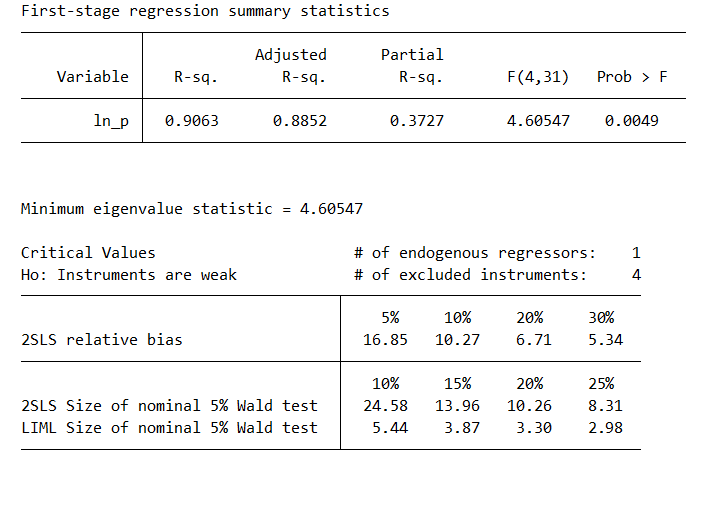
\includegraphics[width=0.7\textwidth]{fig/result_11-11-e.png}
    \end{figure}
    一般選用 F>10 作為好的 IV 的標準 --- 無法拒絕是一個弱IV
\end{frame}


\begin{frame}[fragile]
    \frametitle{另類檢驗法}

    也可以土法煉鋼去檢驗
    \begin{lstlisting}
reg ln_p ln_pf time qprod_l lexpts_l ln_y ln_pb popgro 
test ln_pf time qprod_l lexpts_l \end{lstlisting}
    
        \begin{block}{第一階段的變數}
            在進行第一階段估計時,除了工具變數以外,其他外生變數也要一併納入估計。
            
            而檢驗則只需要做工具變數的聯合檢定。
        \end{block}
\end{frame}

\begin{frame}
    \frametitle{時間序列上的現象}
    老師跳過了時間序列的部分,透過這題稍微補充。

    \begin{figure}
        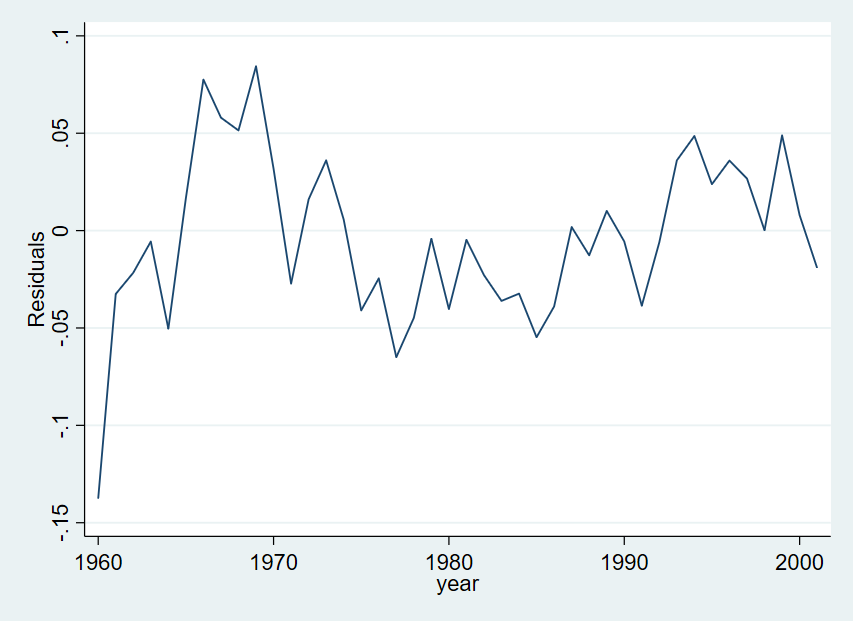
\includegraphics[width=0.75\textwidth]{../Results/11-11_AC.png}
        \caption{殘差項的折線圖}
    \end{figure}
    
\end{frame}

\begin{frame}
    \frametitle{時間序列上面的變異數異質性}

    異質性
    \begin{itemize}
        \item $e_i \sim \mathcal{N}(0, \sigma_i^2), \sigma_i^2 = h(x_i\beta)$
        \item $e_t = \rho e_{t-1} + \nu_t$
    \end{itemize}

    兩種都違反 OLS 的假設,第二種 $cov(e_t, e_{t-1})\ne 0$,稱為自相關 (autocorrelation)。
    這時模型出現了自相關誤差(autoregressive error)。
\end{frame}

\begin{frame}[fragile]
    \frametitle{自相關誤差解決方法}

    與一般異質性問題類似,可以兩種做法
    \begin{enumerate}
        \item 將錯就錯,但好好把有自相關時的變異數計算出來 --- Heteroskedasticity and Autocorrelation Consistent(HAC) Standard Error
        \item 將變數做改變 --- GLS
    \end{enumerate}

    \vfill

    以這題為例,示範計算兩階段估計時,遇到有自相關的時候的穩健做法 --- HAC 穩健標準誤差。
    
    \begin{lstlisting}
ivregress 2sls ln_q (ln_p = ln_pf time qprod_l lexpts_l) ln_y ln_pb popgro, ///
vce(hac nw 2) first \end{lstlisting}
\end{frame}

\begin{frame}[fragile]
    \frametitle{Newey-West HAC 標準誤差}
\begin{lstlisting}
ivregress 2sls ln_q (ln_p = ln_pf time qprod_l lexpts_l) ln_y ln_pb popgro, ///
vce(hac nw 2) first \end{lstlisting}
    \begin{itemize}
        \item 指令中的 \texttt{vce} 告訴 Stata 要特別計算標準誤差。
        \item \texttt{hac} 表示要考慮異質性(heteroskedasticity)與自相關(autocorrelation)的問題
        \item \texttt{nw} 表示要用 Newey-West (1987) 的計算方法(不用管)
        \item \texttt{2} 表示在考慮自相關時,要考慮兩期的落後,也就是 $e_t = \rho_1 e_{t-1} + \rho_2 e_{t-2} + \nu_t$。期數選擇超出範圍
        \item 如果不指定數字,就是用 N-2期 lag (容易over fit)
    \end{itemize}
    
\end{frame}

\begin{frame}
    \frametitle{視覺化殘差像之間的自相關}
    一般來說會有兩種
    \begin{itemize}
        \item Autocorrelation function --- 
        
        \begin{equation*}
            \frac{corr(y_t, y_{t+h})}{\sqrt{var(y_t) var(y_{t+h})}}
        \end{equation*}
        \begin{equation*}
            y_t = {\color{red} \hat{\rho}^{AC}_{t-k}} y_{t-k} + \mu_t
        \end{equation*}
        \item Partial autocorrelation function --- 
        \begin{equation*}
            \frac{corr(y_t , y_{t+h} \given y_{t\dots t+h-1} )}{\sqrt{var(y_t\given y_{t\dots t+h-1})var(y_{t+h}\given y_{t\dots t+h-1})}}
        \end{equation*}
        \begin{equation*}
            y_t = \alpha + \alpha_1 y_{t-1} +\alpha_2 y_{t-2} + \dots + {\color{red} \hat{\rho}^{PAC}_{t-k}} y_{t-k} +  + \mu_t
        \end{equation*}
    \end{itemize}

    選不同的 $h$ ,都有對應的 AC, PAC,可以連同標準誤差畫出來

\end{frame}

\begin{frame}
    \begin{figure}
        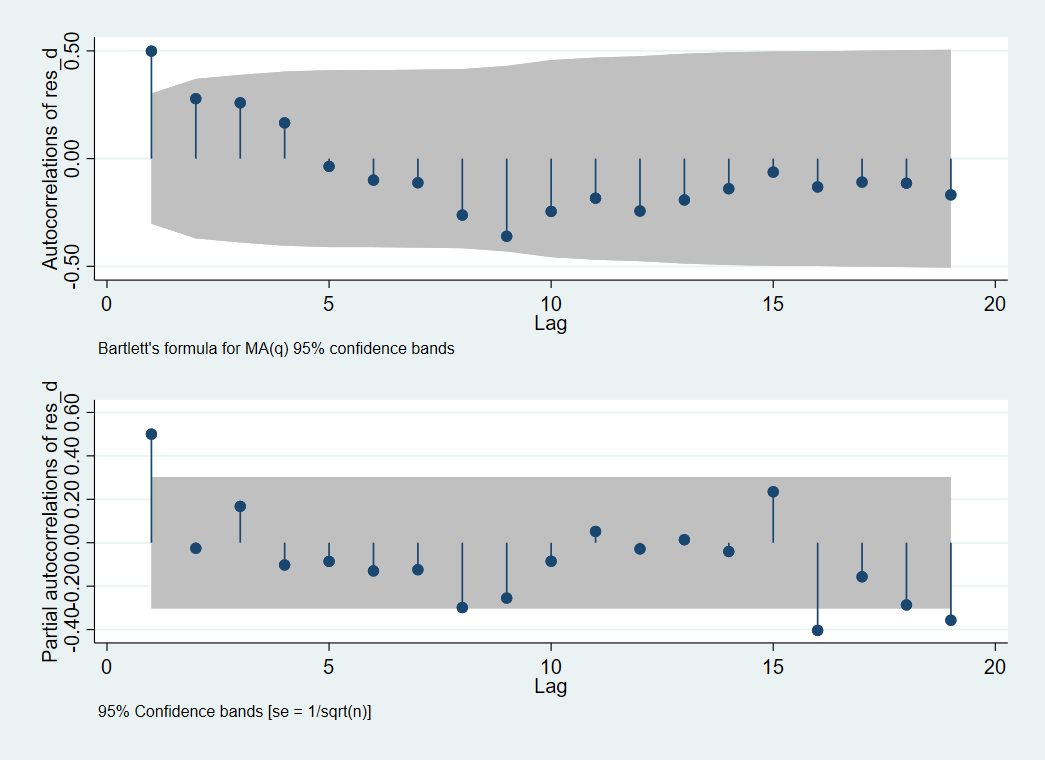
\includegraphics[width=\textwidth]{../Results/ac pac.png}
    \end{figure}
\end{frame}